\documentclass[12pt,a4paper]{article}
\usepackage[swedish,english]{babel}
\usepackage[T1]{fontenc}
\usepackage[utf8]{inputenc}
\usepackage{graphicx}
\usepackage{mathtools}
\usepackage{subcaption}
\usepackage{float}

\graphicspath{ {images/} }

\author{
  Matstoms, Axel
  \and
  Jankovi\'{c}, Luka
  \and
  Matstoms, Ivar
}

%\date{2018-03-15}

\title{GAMLP: En symbolhanterare}

\begin{document}
\selectlanguage{swedish}
\maketitle
\begin{figure}[h]
  \centering
  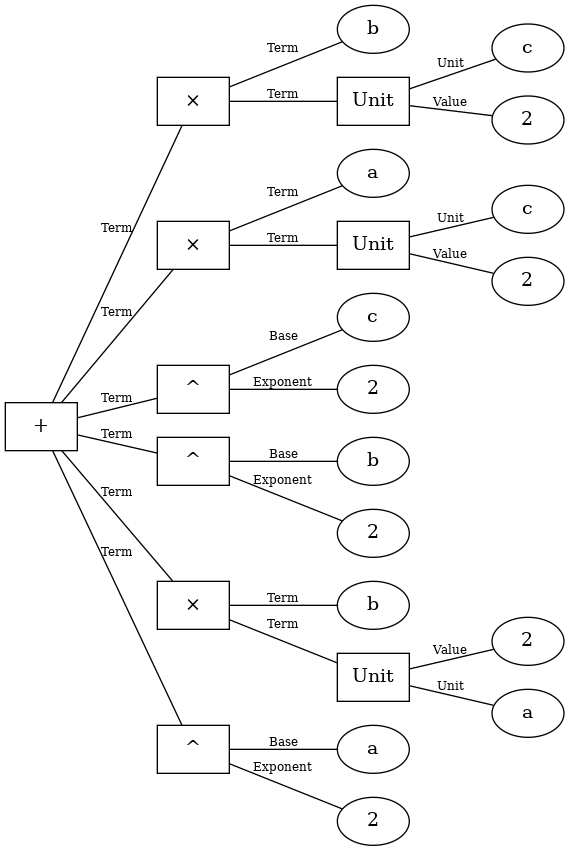
\includegraphics[width=0.7\textwidth]{image27}
  %\caption{Välj en olämplig bild}
\end{figure}
\newpage
\selectlanguage{english}
\begin{abstract}
The purpose of this project is to look at some of the techniques used by sites such as WolframAlpha to simplify algebraic expressions and solve particular kinds of equations. To research this we wrote an application in Python with some of the features of such sites.  We chose to work with Python because of how quickly code can be written in Python and due to the fact everybody in the group knew Python before the project even started. During the span of this project we were able to develop an application which is able to take input and construct an abstract syntax tree which is then simplified. The application is able to handle many of our goals set in the beginning, including addition and multiplication of polynomials correctly, although not always fully simplified. The application is also able to solve polynomials up to the second degree. With time the application could easily be expanded to cover more aspects of what we set out to do such as polynomial division and solving polynomial equations of higher grades.ga
\end{abstract}
\textbf{Keywords:} Abstract syntax tree; Python; Algebraic Expressions
\selectlanguage{swedish}
\newpage
\tableofcontents
\newpage
\section{Inledning}
Eftersom vi alla i gruppen delar en stor passion för programmering ville vi göra något som kombinerar programmering med ett naturvetenskapligt ämne. Vi övervägde flera olika projekt, bland annat en realtids fysikmotor, implementationer av matematiska funktioner (såsom sinus, exponenter) på hårdvarunära nivå samt idén som valdes: en symbolhanterare. En symbolhanterare, eller CAS, Computer Algebra System, är ett datorprogram som kan mata in, tolka, och lösa ekvationer, exempelvis \(5x + 10 = 20\). En annan funktion som en symbolhanterare antar är förmågan att förenkla uttryck, exempelvis \((x + 2)(x - 3) \Leftrightarrow (x^{2} - x - 6)\). Skillnaden mellan en vanlig miniräknare och en symbolhanterare är att symbolhanterare förstår algebra och kan samt kan hantera variabler, inte bara värden.
\section{Teori}
\subsection{Abstrakt syntaxträd}
Det är besvärligt för ett program att tolka ekvationer som är skrivna på vanlig form (e.x. \(5x + 10 = 15\)). Därför är det viktigt att ekvationen först byggs upp på ett sätt som är mer hanterbart för ett datorprogram. Så kallade abstrakta syntaxträd används oftast inom datavetenskap för att strukturera programmeringskod så att en kompilator kan omvandla källkoden till ett exekverbart program. Men på grund av likheterna mellan programmeringsspråkens syntax och matematiska ekvationer användes abstrakta syntaxträd i detta arbete.
\subsubsection{Allmänt om träd}
Inom datavetenskap beskrivs träd som en form av datastruktur för att representera hierarkisk data. Ett träd inom matematiken består av noder som är sammansatta på så vis att varje nod kan innefatta ett eller flera barn, som i sig också är noder. I det här dokumentet kallas barnen för barnnoder eller subnoder. Noder behöver dock ej innefatta några barn, och då kallas dessa noder för löv. Dock behöver varje nod anta ett värde. Detta kan vara t.ex. ett numeriskt värde (e.x. \(5\) eller \(10\)), eller en operation (e.x. addition, multiplikation). Om en nod ej är ett barn till en annan nod betyder det att denna nod är högst upp i trädet. Denna typ av nod kallas för rotnod eller bara rot.
\subsubsection{Implementation av syntaxträd}
Trädet i sig utgår från en rotnod (eng. rootnode). I vårt fall är denna nod alltid ett likhetstecken (\(=\)), eftersom det är där ekvationen utgår ifrån. Precis som t.ex. en operatörsnod kan rotnoden anta två subnoder (I detta fall måste två noder antas, en för VL och en för HL). Därefter kan leden byggas upp av olika sorters noder.
\subsubsection{Noder}
\label{subsubsec:noder}
En nod måste anta ett värde. Detta kan uppnås genom att ge noden ett konkret värde (e.x. \(5\) eller \(10\)), en konstant (e.x. \(\pi\), \(e\)), funktion (e.x. \(log\), \(sin\)) eller operator (e.x. \(+\), \(-\), \(\times\), \(\div\), \string^). Om noden är sådan att den kräver argument, dvs. kräver ett eller flera värden för att själv få ett värde (\(+\) har ej ett värde utan två siffror på vardera sida av sig.) så kan noden själv anta noder (s.k. barnnoder, eng. childnodes) för att uppfylla sitt värde. Se Figur \ref{fig:2131}.
\begin{figure}[h]
  %24
  \centering
  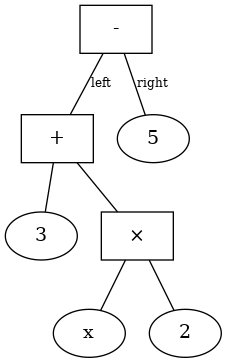
\includegraphics[width=0.3\textwidth]{image24}
  \caption{Visuell representation av \((2x + 3) - 5\) som ett abstrakt syntaxträd.}
  \label{fig:2131}
\end{figure}
Eftersom programmet ska kunna hantera ekvationslösning, måste den okända variabeln kunna representeras (e.x. \(5x + 10 = 20\). Här är \(x\) den okända variabeln). För att representera variabeln används en speciell typ av nod; så kallad enhetsnod. Denna nod antar ett värde (för koefficienten) och en representation av den okända variabeln; en så kallad enhet. Denna enhet består av själva variabeln och vilken grad som den representeras i. Se Figur \ref{fig:2132} för en visuell representation av \(2x^{2}\) som en enhetsnod.
\begin{figure}[h]
  %25
  \centering
  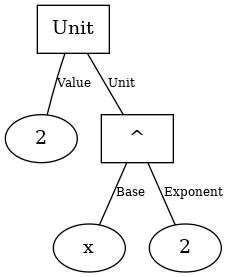
\includegraphics[width=0.3\textwidth]{image25}
  \caption{\(2x^{2}\) representerat som en enhetsnod med enheten \(x^{2}\) och värdet \(2\).}
  \label{fig:2132}
\end{figure}
\subsection{Allmänt om förenkling}
Operatörsnoder vars subnoder endast består av numeriska värden räknas helt enkelt ihop med den operatorn som noden representerar. Då kommer denna operatörsnod ersättas med en nummernod som antar det ihopräknade värdet.
\subsection{Homogena noder}
\label{subsec:homogena}
Homogena noder är de noder där ordningen av subnoder ej spelar någon roll vilket gör att de kan lagras som en lista (array) och är inte limiterad i antal. Dock byggs homogena noder först upp av flera noder med bara två subnoder (Se \ref{subsec:inhomogena_noder} Inhomogena noder) eftersom det är så programmet tolkar inmatningen, se Figur \ref{fig:2311}.
\subsubsection{Allmän förenkling av homogena noder}
\label{subsubsec:förenkling_homogena}
\begin{figure}[h!]
  %22
  \centering
  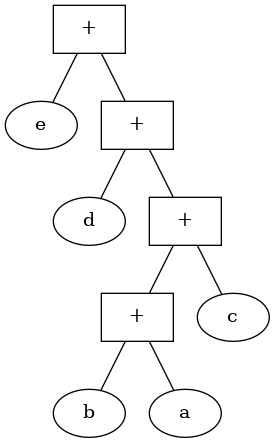
\includegraphics[width=0.3\textwidth]{image22}
  \caption{\((a + b + c + d + e)\) tolkat av programmet.}
  \label{fig:2311}
\end{figure}
Att förenkla noder som precis har tolkats av programmet (se Figur \ref{fig:2311}) är dock opraktiskt. Därför är det första steget i förenklingen att försumma staplade homogena noder av samma typ till en enda nod. Om noderna antar numeriska värden räknas de ihop till en subnod, medans variabler (\(x\)) helt enkelt lämnas som en subnod. Efter det läggs elementen in i noden en efter en och varje element kontrolleras om den kan slås ihop med en annan subnod. Detta gäller dock endast för noder med numeriska värden. Hur enhetsnoder (se \ref{subsubsec:noder} för förklaring av enhetsnod) hanteras är dock olika för varje typ av homogen nod. Därför förklaras detta i detalj i samband med varje typ av nod.\par
Två enhetsnoder med samma enhet kan slås ihop genom att addera värderna.
\begin{figure}[h!]
  %16
  \centering
  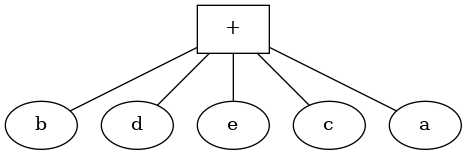
\includegraphics[width=0.5\textwidth]{image16}
  \caption{\((a + b + c + d + e)\) efter första steget av förenkling av homogen nod}
  \label{fig:2312}
\end{figure}
\begin{figure}[h]
%  \begin{subfigure}[h]
%    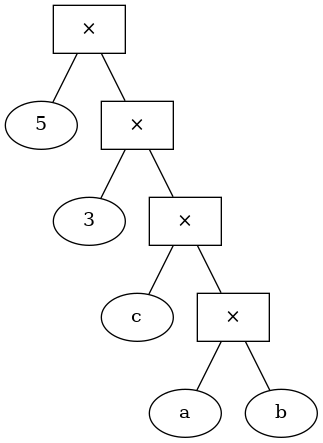
\includegraphics[width=0.3\textwidth]{image23}
%  \end{subfigure}
%  \begin{subfigure}[h]
%    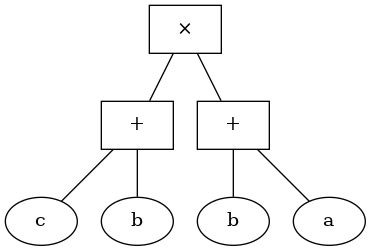
\includegraphics[width=0.3\textwidth]{image26}
%  \end{subfigure}
%  \begin{subfigure}[h]
%    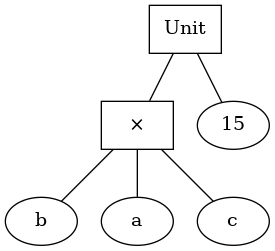
\includegraphics[width=0.3\textwidth]{image19}
%  \end{subfigure}
  \centering
  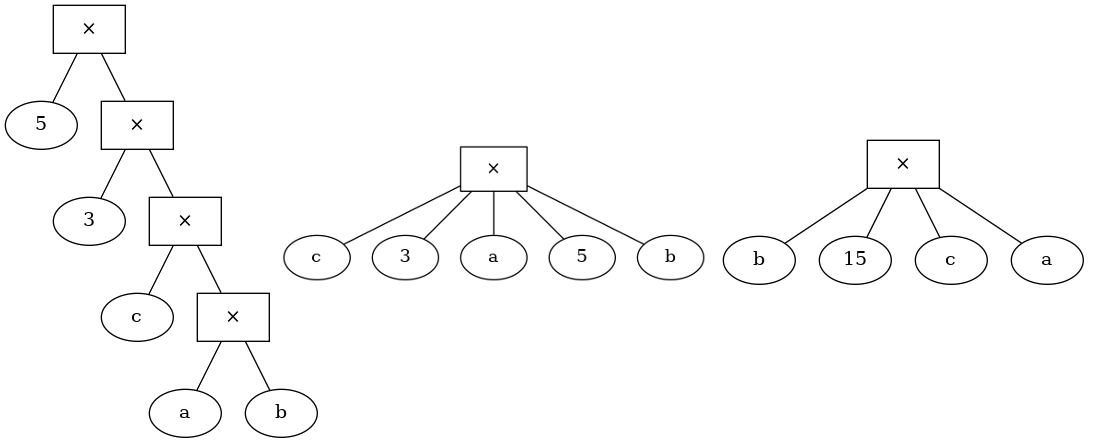
\includegraphics[width=0.9\textwidth]{image-merged}
  \caption{\((a \times b \times c \times 3 \times 5)\) förenklas i tre steg, a,b,c lyfts upp till samma nod och talen separeras till sin egen nod, tillslut räknas talen ihop.}
  \label{fig:2313}
\end{figure}
\subsubsection{Additionsnod}
Förenklingen av en additionsnod funkar genom att fylla på en tom lista med värden från en additionsnods barnnoder och kollar om en nod i barnnodslistan kan läggas ihop med en nod i den nya listan. T.ex. om en additionsnod består av bara siffernoder så kommer dessa adderas. Om flera enhetsnoder med samma enhet förekommer så kommer deras koefficienter summeras (se Figur \ref{fig:2321}). En potensnod kan slås ihop med en annan nod om basen på potensnoden är samma som den andra noden, isåfall skapas en ny potensnoden med exponenten ökad med ett.
\begin{figure}[h!]
  \centering
  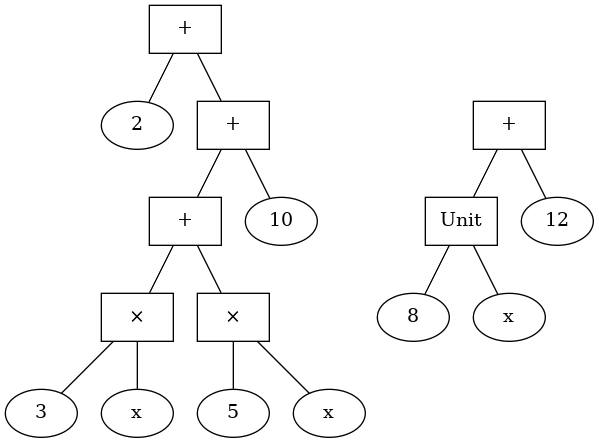
\includegraphics[width=0.7\textwidth]{image-merged2}
  \caption{\(5x + 3x + 10 + 2\) förenklas till \(8x + 12\)}
  \label{fig:2321}
\end{figure}
\subsubsection{Multiplikationsnod}
Efter de generella förenklingarna av homogena noder (Se \ref{subsubsec:förenkling_homogena} Allmän förenkling av homogena noder) separeras additionsnoder från övriga noder. Alla kombinationer av dessa separerade additionsnoders subnoder multipliceras med övriga noder och adderas ihop. Enhetsnoder kombineras genom att skapa en ny enhetsnod vars koefficient består av produkten av de originala enhetsnodernas koeficienter och vilken grad den nya enhetsnoden representeras i bestäms av hur många enhetsnoder det från början var. (e.x. \(5x \times 10x = 50x^{2}\)). Enhetsnoder kan också kombineras med övriga noder genom att de övriga värdena multipliceras in i enhetsnodens värde (Se \ref{subsubsec:noder} Noder).
\begin{figure}[h!]
  %26
  %32
  \centering
  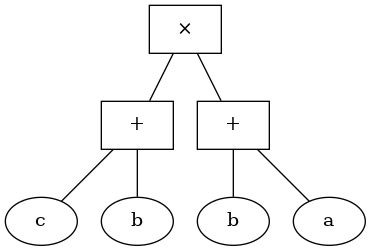
\includegraphics[width=0.4\textwidth]{image26}
  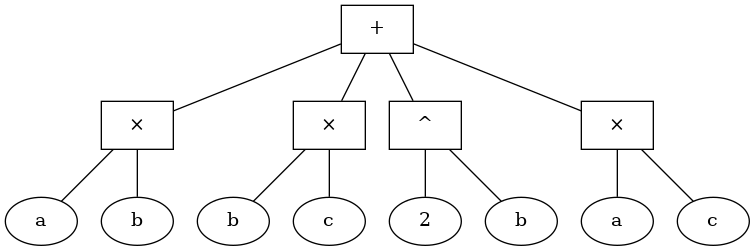
\includegraphics[width=0.8\textwidth]{image32}
  \caption{\((a + b) * (c + b)\) förenklas till \((a * b) + (b * c) + (b ^ 2) + (a * c)\)}
\end{figure}
\subsection{Inhomogena noder}
\label{subsec:inhomogena_noder}
Inhomogena noder genomför inhomogena operationer; dvs. operationer som där ordningen av subnoderna spelar roll. (e.x. \(a - b \neq b - a\)). Därmed kan inhomogena noder ej kombineras rekursivt på samma sätt som homogena noder kan. (Se \ref{subsubsec:förenkling_homogena} Allmän förenkling av homogena noder) Detta medger också att det inte finns ett allmänt sätt att förenkla inhomogena noder.
\subsubsection{Potensnod}
Potensnoder innehåller två barnnoder, basen och exponenten. En potensnod med en additionsnod i basen, exempelvis \((a+b+c)^{3}\), expanderas med hjälp av multinomialsatsen. Som man kan ana på namnet liknar multinomialsatsen binomialsatsen. Skillnaden är att multinomialsatsen är ett mer generaliserat sätt att beskriva utveckling av polynom, och är alltså ej begränsad till endast binom. Satsen lyder
\[(a_{1}+a_{2}+\ldots+a_{m})^{n}=\displaystyle\sum_{k_{1}+\dots+k_{m}=n}\binom{n}{k_{1},k_{2},\dots,k_{m}}a_{1}^{k_{1}}\cdot\ldots\cdot a_{m}^{k_{m}}\]
Den behöver dock lite förklaring. Med \(\displaystyle\sum_{k_{1}+\dots+k_{m}=n}\) menas alla möjliga kombinationer med återläggning av exponenter i \(a_{1}^{k_{1}}\cdot a_{2}^{k_{2}}\cdot\ldots\cdot a_{m}^{k_{m}}\) där \(\displaystyle\sum_{i=0}^{m}k_{i}=n\) uppfylls. Vidare behöver  \(\binom{n}{k_{1},k_{2},\ldots,k_{m}}\) förklaras. Detta kallas för \textit{multinomialtal} eller \textit{multinomialkoefficient}, som i sig en generalisering av binomialkoefficienten \(\binom{n}{k}\). Multinomialkoefficienten kan skrivas om på detta vis.
\[\binom{n}{k_{1},k_{2},\ldots,k_{m}}=\frac{n!}{k_{1}!\cdot k_{2}!\cdot\ldots\cdot k_{m}!}\]
\subsubsection{Subtraktionsnod}
Subtraktionsnoden är ej en homogen nod då ordningen på ekvationen spelar roll \(a-b\neq b-a\) och därmed måste subtraktionsnoden anta endast två noder; en för vänster sida och en för höger sida. För att simplifiera subtraktions noden så implementeras inget nytt. Den använder sig istället av additions noden och multiplikations noden för att uppnå en minus operation. Istället för att direkt räkna ut \(a-b\) så skrivs ekvationen om till \(a+((-1)\cdot b)\). Därmed kan samma resultat uppnås med bara addition och multiplikation.
\begin{figure}[h!]
  \centering
  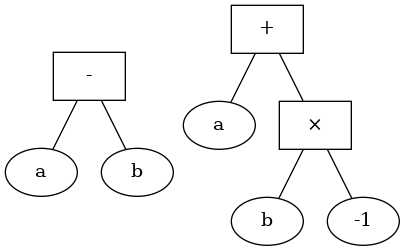
\includegraphics[width=0.4\textwidth]{image-merged3.png}
  \caption{\(a-b\) före och efter förenkling. Minus noden transformeras till en additionsnod med b ersatt med \(b*-1\)}
\end{figure}
\subsubsection{Divisionsnod}
På samma sätt som subtraktionsnoden skiver om ekvationen \(a-b\Rightarrow a+((-1)*b)\) så skriver divisionsnoden om ekvationen så att förenklingen istället kan hanteras av multiplikationsnoden. \(a/b\Rightarrow a*(b^{-1})\)
\begin{figure}[h!]
  \centering
  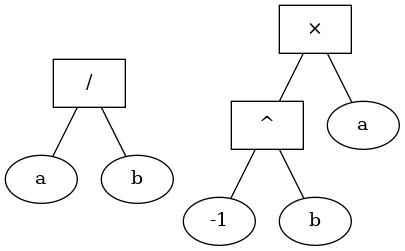
\includegraphics[width=0.4\textwidth]{image-merged4.png}
  \caption{\(a/b\) förenklas till \(a*(b^{-1})\)}
\end{figure}
\subsubsection{Ekvationsnod}
En ekvationsnod antar en nod för varje led (I vårt projekt kan en ekvationsnod endast anta två subnoder; en för VL och en för HL.) Målet med ekvationsnoden är att representera en ekvation som kan lösas ut och förenklas. Detta innebär att subtrahera ett led från båda leden, som på så sätt lämnar ett led tomt.
\begin{figure}[h!]
  \centering
  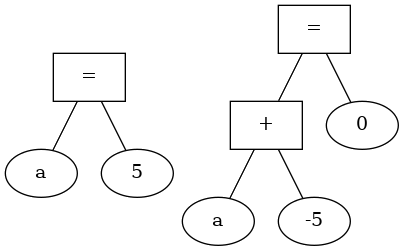
\includegraphics[width=0.4\textwidth]{image-merged5.png}
  \caption{\((x+4)\cdot (2+x)=10\) förenklas till \(-2-10=0\)}
\end{figure}
\subsection{Ekvationslösning}
Att lösa ekvationer med en okänd (dvs. lösa ut x) innebär att först förenkla ekvationen så att en sida antar värdet 0. Därefter kommer olika regler appliceras på ekvationen beroende på vilken grad den är i. Vilken grad den är i bestäms av den högsta potensen.

När en ekvation löses så förenklas den först så högerled är lika med 0. Sen går den igenom alla direkta subnoder nod för nod och kolla efter okända och potens. GAMLP kan bara lösa ekvationer med en okänd. Den högsta exponenten på den okända är graden på ekvationen. Programmet har en samling av olika metoder för att lösa ekvationer och hittar den lämpligaste metoden och utför den. Vilka metoder som används beskrivs i \ref{subsubsec:Ekvationsmetoder}.
\subsubsection{Ekvationsmetoder}
\label{subsubsec:Ekvationsmetoder}
\paragraph{Förstagradsekvationer}
\(kx+m=0\Leftrightarrow x=\frac{-m}{k}\)
\paragraph{Andragradsekvationer}
\(ax^{2}+bx+c=0\Leftrightarrow x=-\frac{b}{2a}\pm \sqrt{\frac{b^{2}}{(2a)^{2}}-\frac{c}{a}}\)
\paragraph{Enkla exponensialekvationer}
\(a\cdot x^{b}+k=0\Leftrightarrow x=(\frac{-k}{a})^{\frac{1}{b}}\)
\section{Metod}
\subsection{Klasser och Objekt}
\label{subsection:klasserochobjekt}
En viktig del av struktureringen av noder (se \ref{subsubsec:noder}, Noder) handlar om att en nod kan vara en utökad typ av en annan nod. Det vill säga, istället för att på nytt skapa varenda nod kan man istället skapa en generell nod för t.ex. operatörer, och sedan utöka den för varje sorts operation. Detta kallas för Objektorienterad Programmering (Object Oriented Programming, OOP). 
\subsubsection{Objektorienterad programmering}
I princip funkar Objektorienterad programmering genom att man för varje föremål, struktur, etc. man vill beskriva i ett program har en s.k. klass. En klass är en abstrakt modellering av ett objekt; dvs. den innehåller definitioner för attributer och handlingar. (Kan liknas t.ex. en ritning; klassen innehåller information om strukturen, men är i sig inte en färdig produkt.). Sedan används klassen för att skapa objekt som kan fylla på med värden på attributerna och faktiskt utföra de beskrivna handlingarna. Ett exempel som är enkelt att förstå är att föreställa sig klassen Bil. I denna klass är det definierat att varje bil har t.ex en färg, maxhastighet, osv. Den har också vissa handlingar (alt. metoder) beskrivna; man kan köra bilen, tanka den, osv. Detta är beskrivningen av klassen Bil, och det är väldigt viktigt att komma ihåg att klassen, dvs. definitionen av bilen i sig ej är en bil. Istället skapas en instans av klassen bil; alltså kan man säga att objektet är skapat med klassen som ritning. Vi återvänder till Bil-exemplet och skapar ett objekt; en bil med färgen blå och maxhastighet 200 km/h. Denna teoretiska bil kan nu köras, tankas osv.
\subsubsection{Subklasser och arv}
Ett användbart redskap inom objektorienterad programmering är arv. För att fortsätta med bil-exemplet (se \ref{subsection:klasserochobjekt} Klasser och Objekt) kan vi säga att klassen Bil är en subklass (dvs ärver från) klassen Fordon. Klassen Bil har då alla attributer och metoder som klassen Fordon har samt attributer och metoder som läggs till i definitionen av Bil. Klassen fordon kan exempelvis ha attributerna kan-flyga och bränsle-typ. Därmed kan en instans av klassen Bil anta värden för dessa attributer.
\subsubsection{Noder}
Alla noder är subklasser av klassen Nod. Nodklassen innehåller definitioner för metoder som används av och är gemensamma för alla subklasser. T.ex. så hanteras operationer av noder (e.x. addition, subtraktion) av denna klass (se tabell \ref{tab:basenodefunc}). Alla operatörsnoder är subklasser av klassen operatörsnod. Operatörsnoden har dock ingen funktion i sig, utan används för att enklare urskilja vilka noder som är operatörsnoder och vilka som inte är. Därefter grupperas additionsnodens och multiplikationsnodens klass som var sin subklass av klassen honomgen operatörsnod. Detta gjordes eftersom både multiplikationsnoden och additionsnoden är homogena noder (se \ref{subsec:homogena}
Homogena noder är de noder där ordningen av subnoder ej spelar någon roll vilket gör att de kan lagras som en lista (array) och är inte limiterad i antal. Dock byggs homogena noder först upp av flera noder med bara två subnoder (Se \ref{subsec:inhomogena_noder} Inhomogena noder) eftersom det är så programmet tolkar inmatningen, se Figur \ref{fig:2311}.
\begin{figure}[h!]
  \center
  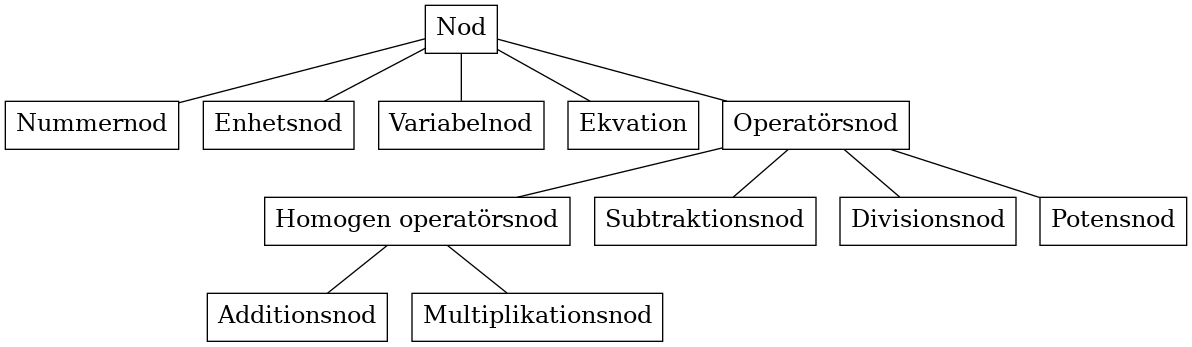
\includegraphics[width=1\textwidth]{image20}
  \caption{Diagram av nodklassen samt dess alla subklasser.}
\end{figure}

\begin{figure}[h!]
  \centering
  \begin{tabular}{l|p{10cm}}
    \textbf{Namn} & \textbf{Användning} \\
    \hline
    \texttt{hash\_node} & Returnerar ett unikt nummer för just denna nod som används för att identifiera den. \\
    \texttt{get\_children} & Returnerar subnoder. \\
    \texttt{get\_int\_value} & Om noden går att räkna ut och resultatet är ett heltal returnera heltalet. \\
    \texttt{latex} & Returnerar en latex representation. \\
    \texttt{simplified} & Bygger upp en nod som är en förenkling av sig själv. \\
    \texttt{eval} & Räknar ut värdet på en nod. \\
    \texttt{eq} & Jämför noder (samma struktur, variabler etc.) \\
    \texttt{formatted} & Returnerar en text representation av noden.
  \end{tabular}
  \captionof{table}{Funktioner och dess användning i basklassen nod.} \label{tab:basenodefunc}
\end{figure}

\subsection{Tolkning av inmatade ekvationer}
För att läsa in uttryck på normal form och för att enkelt omvandla de till abstrakta syntaxträd krävs en lexikalisk analys av den inmatade datan som sedan tolkas av en parser. Att hantera lexikalisk analys och att utveckla en parser ligger utanför projektet. Därför användes biblioteket purplex, som utför denna lexikaliska analys och har en inbyggd parser.

\subsubsection{Lexikalisk analys}
En lexer separerar den inmatade datan till s.k. tokens baserat på fördefinierade mönster och bygger upp en array (lista) baserad på dessa tokens. Med andra ord letar en lexer efter ett sorts mönster i indatan och fyller på array-en med motsvarande tokens. Tokens känns igen med hjälp av mönstermatchningsspråket regex. Nedan visas en tabell över vilka mönster som letas efter och vad de ersätts med i listan i den lexikaliska analysen. 
Exempel: \(5x+10=20\Rightarrow\) ([värde, 5], [okänd \(x\)], [addition], [värde, 10], [likhetstecken], [värde, 20])

\end{document}
